\subsection{Practical Application Performance}
\label{socksdirect:subsec:application}

This section demonstrates that \sys {} can significantly improve the performance of actual applications without modifying the code.
Rsocket~ \cite {rsockets} is not compatible with any of the following applications.

\subsubsection{Nginx HTTP Server}

To test the typical web service scenario where the client comes from the network and provides services within the host, this section uses Nginx~ \cite {nginx} v1.10 as a reverse proxy between the HTTP request generator and the HTTP response generator.
Nginx and the response generator are located in the same host, while the request generator is located in a different host.
The generator communicates with Nginx using keep-alive TCP connections.
Due to fork, LibVMA~ \cite {libvma} cannot be used with unmodified Nginx.
In Figure \ref {socksdirect:fig:eval-nginx}, the request generator measures the time from sending the HTTP request to receiving the entire response.
For smaller HTTP response sizes, compared with Linux, \sys {} can reduce latency by 5.5 times.
For large responses, due to zero-copy, \sys {} can reduce latency by up to 20 times.

\begin{figure}[htbp]
	\centering 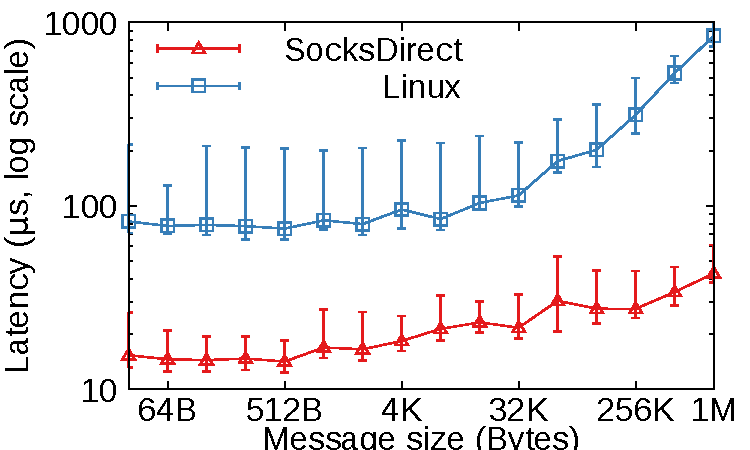
\includegraphics[width=0.5\textwidth]{eval/web/msgsize-clocal-lat.pdf}
	
	\caption{Nginx HTTP request end-to-end latency.}
	\label{socksdirect:fig:eval-nginx}
\end{figure}

\subsubsection{Redis Key-Value Store}

This section uses the redis-benchmark client and 8-byte GET requests to measure the latency of the Redis~ \cite {redis} in-memory key-value store server.
When using Linux, the average latency is 38.9 $ \mu s $, and the 1% and 99% percentile latencies are 31.6 and 56.1 $ \mu s $ respectively.
After using \sys {}, the average latency is 14.1 $ \mu s $ (64% lower than Linux), and the 1% and 99% percentiles are 8.4 and 19.1 $ \mu s$.

\subsubsection{Remote Procedure Call (RPC) Library}

This section uses RPClib~ \cite {rpclib} to measure RPC latency.
Running example 1~KiB RPC in two processes within the host with RPClib takes 45 $ \mu $s. On two hosts, RPC takes 79 $ \mu$s.
Using \sys {}, the intra-host latency becomes 21 $ \mu s $ (a reduction of 53%), and the inter-host latency is 46 $ \mu$s (a reduction of 42%).

However, \sys{} is not a panacea. Even with \libipc{}, the performance of RPClib is still far below that of the most advanced RPC libraries, such as eRPC \cite{kalia2018datacenter}, due to the overhead of RPClib becoming a performance bottleneck.

\subsubsection{Network Function Pipeline}

64-byte data packets in \emph{pcap} format come from an external packet generator, pass through the Network Function (NF) pipeline, and are sent back to the packet generator.
This section implements each NF as a process, which inputs packets from \emph{stdin}, updates local counters, and outputs to \emph{stdout}.
For Linux, \emph{pipe} and \emph{TCP socket} are used to connect NF processes within the host.
Figure \ref{socksdirect:fig:eval-tun-tput} shows that the throughput of \sys{} is 15 times and 20 times that of Linux pipe and TCP socket, respectively.
It even approaches the most advanced NF framework, NetBricks~\cite{panda2016netbricks}.

\begin{figure}[htbp]
	\centering
	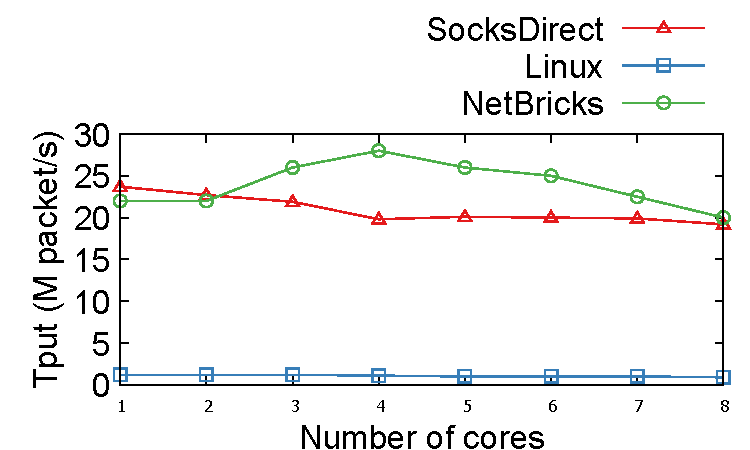
\includegraphics[width=0.5\textwidth]{eval/microbenchmark/nfv-tun-tput.pdf}
	
	\caption{Throughput of network function pipeline.}
	\label{socksdirect:fig:eval-tun-tput}
	%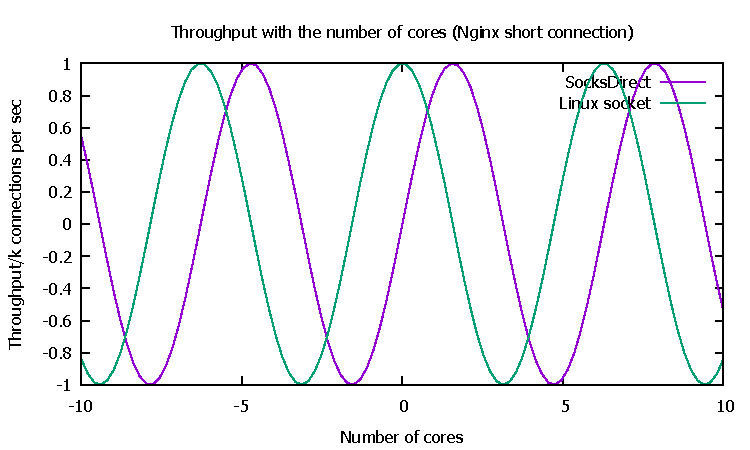
\includegraphics[width=\textwidth]{eval/microbenchmark/nginx-short-tput.pdf}
	%
	%\label{socksdirect:fig:eval-nginx-short}
	%\caption{Nginx throughput.}
	
	%\centering 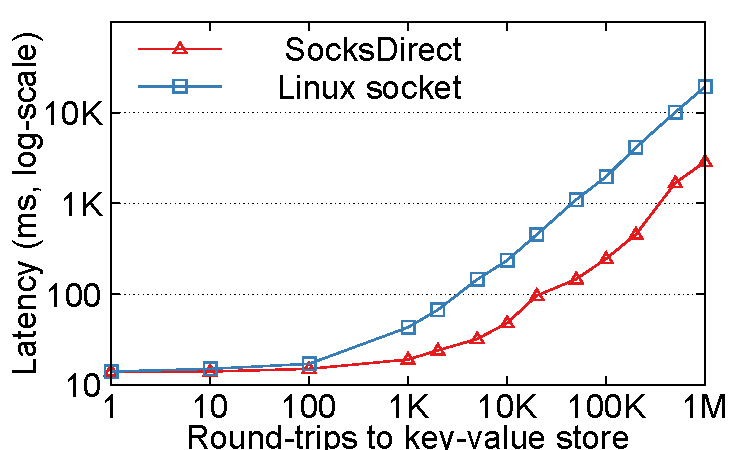
\includegraphics[width=\textwidth]{eval/microbenchmark/nginx-multiround-tput.pdf}
	%
	%\caption{End-to-end HTTP request latency of a web service.}
	%\label{socksdirect:fig:eval-nginx-multiround}
	
	%\centering
	%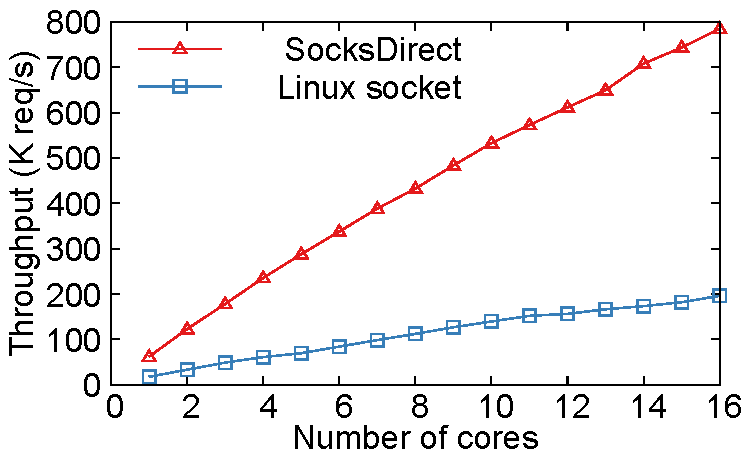
\includegraphics[width=\textwidth]{eval/microbenchmark/corenum-http-tput.pdf}
	%
	%\caption{Multi-core scalability of HTTP backend service throughput.}
	%\label{socksdirect:fig:eval-http-tput}
\end{figure}


%\subsubsection{GraphX on Spark}
%\quad

%Two nodes run distributed PageRank.
%Test elapsed time per iteration with \sys{}, libvma and Linux. (Only need three numbers, no figure.)
